\documentclass[border=12pt]{standalone}
\usepackage{tikz}
\usetikzlibrary{shapes.geometric, arrows.meta, positioning, calc, fit, backgrounds}
\usepackage{fontspec}
\usepackage{amsmath,amssymb}
\setmainfont{DejaVu Sans}

\begin{document}
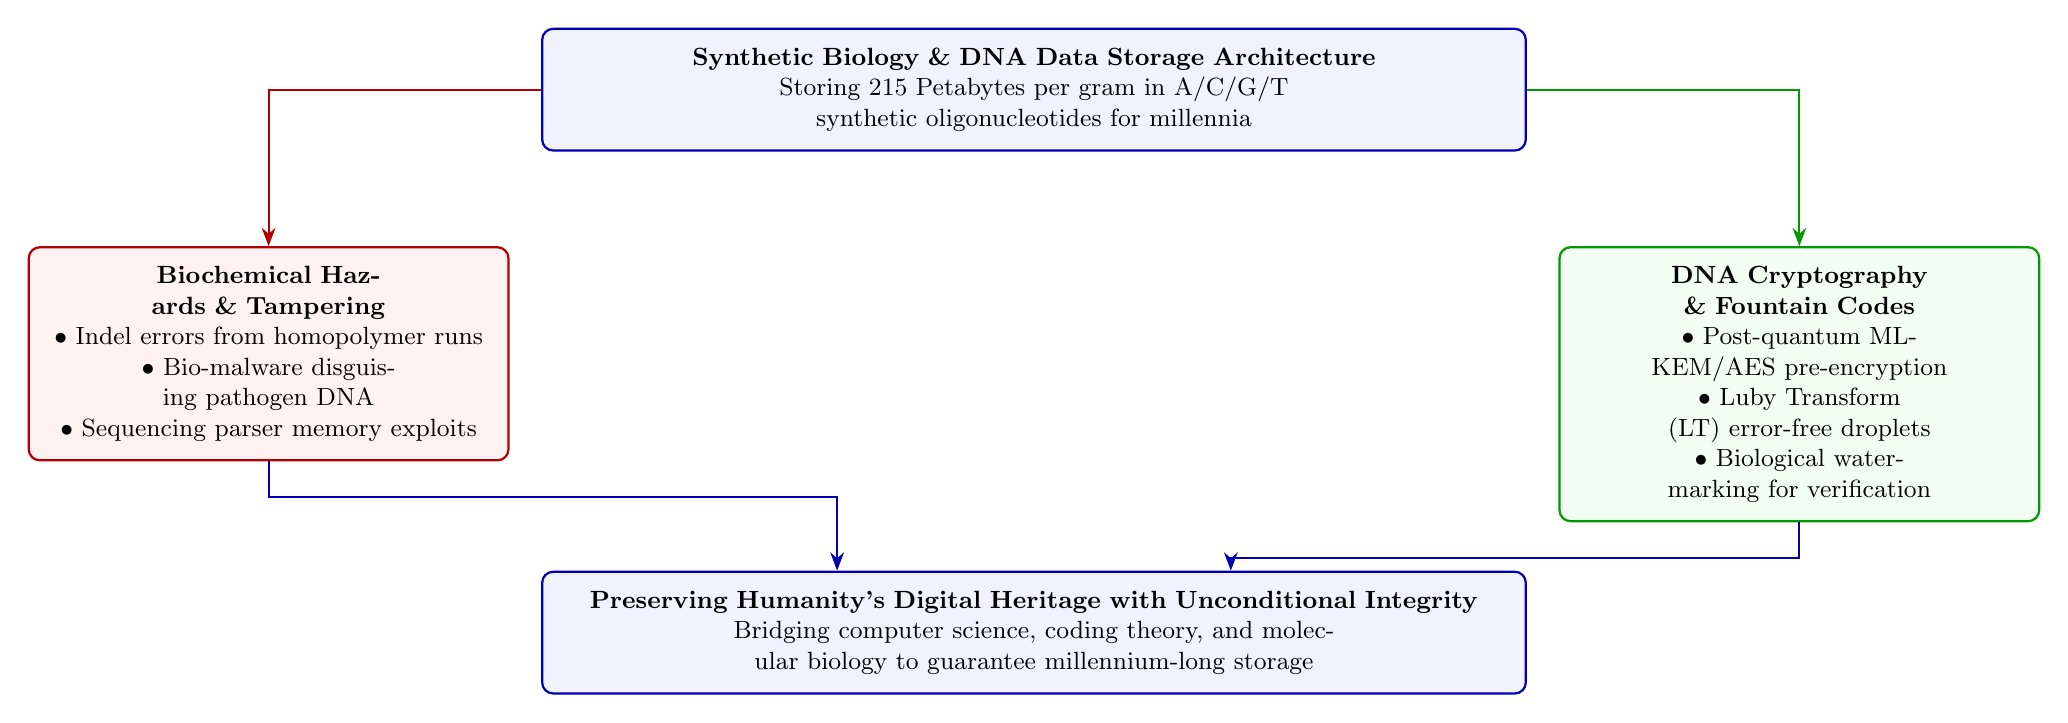
\begin{tikzpicture}[
    font=\small,
    >=Stealth,
    node distance=1.2cm,
    block/.style={rectangle, draw=blue!70!black, fill=blue!5, rounded corners=4pt, thick, align=center, inner sep=7pt},
    alertblock/.style={rectangle, draw=red!70!black, fill=red!5, rounded corners=4pt, thick, align=center, inner sep=7pt},
    greenblock/.style={rectangle, draw=green!60!black, fill=green!5, rounded corners=4pt, thick, align=center, inner sep=7pt},
    amberblock/.style={rectangle, draw=orange!80!black, fill=orange!5, rounded corners=4pt, thick, align=center, inner sep=7pt}
]

\node[block, text width=12cm] (top) {\textbf{Synthetic Biology \& DNA Data Storage Architecture}\\Storing 215 Petabytes per gram in A/C/G/T synthetic oligonucleotides for millennia};

\node[alertblock, below left=1.2cm and 0.4cm of top, text width=5.6cm] (biohazard) {\textbf{Biochemical Hazards \& Tampering}\\$\bullet$ Indel errors from homopolymer runs\\$\bullet$ Bio-malware disguising pathogen DNA\\$\bullet$ Sequencing parser memory exploits};

\node[greenblock, below right=1.2cm and 0.4cm of top, text width=5.6cm] (coding) {\textbf{DNA Cryptography \& Fountain Codes}\\$\bullet$ Post-quantum ML-KEM/AES pre-encryption\\$\bullet$ Luby Transform (LT) error-free droplets\\$\bullet$ Biological watermarking for verification};

\node[block, below=1.0cm of $(biohazard.south)!0.5!(coding.south)$, text width=12cm] (bottom) {\textbf{Preserving Humanity's Digital Heritage with Unconditional Integrity}\\Bridging computer science, coding theory, and molecular biology to guarantee millennium-long storage};

\draw[->, thick, red!70!black] (top) -| (biohazard);
\draw[->, thick, green!60!black] (top) -| (coding);
\draw[->, thick, blue!70!black] (biohazard.south) -- ++(0,-0.45) -| ([xshift=-2.5cm]bottom.north);
\draw[->, thick, blue!70!black] (coding.south) -- ++(0,-0.45) -| ([xshift=2.5cm]bottom.north);

\end{tikzpicture}
\end{document}
